\section{Úloha~č.~3}
\subsection{Zadanie}
Stanovte napětí $U_{R3}$ a proud $I_{R3}$. Použijte metodu uzlových napětí ($U_{A}, U_{B}, U_{C}$).
\begin{table}[H]
\begin{center}
  \begin{tabular}{|c|c|c|c|c|c|c|c|c|}
    \hline
    sk. &  $U [V]$ & $I_{1} [A]$ & $I_{2} [A]$ & $R_{1} [\Omega]$ &  $R_{2} [\Omega]$ &  $R_{3} [\Omega]$ &  $R_{4} [\Omega]$ &  $R_{5} [\Omega]$ \\ \hline
    A & 50 & 0,55 & 0.65 & 525 & 620 & 210 & 530 & 130 \\ \hline
  \end{tabular}
\end{center}
\end{table}
\begin{center}
  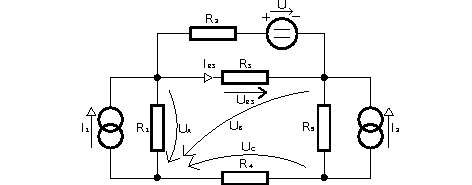
\includegraphics[width=0.8\columnwidth,keepaspectratio]{res/u3o1}
\end{center}

\subsection{Riešenie}
V obvode si premeníme napäťový zdroj $U$ na prúdový zdroj $I$. Ďalej si premeníme rezistory na vodivosti a v obvode si určíme si kde sa nachádza referenčný uzol a zvyšné uzly si označíme písmenami A,~B~a~C. Potom bude obvod vyzerať nasledovne: 
\begin{figure}[H]
\begin{center}
  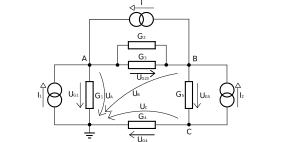
\includegraphics[width=0.8\columnwidth,keepaspectratio]{res/u3o2}
\end{center}
\end{figure}
\noindent
Ďalej si zostavíme rovnice podľa I. Kirchohoffoveho zákona:
\begin{flalign*}
    A:&~I_{1} + I - I_{G23} - I_{G1} = 0 & \\
  B:&~I_{2} + I_{G23} - I - I_{G5} = 0 \\
  C:&~I_{G5} - I_{2} - I_{G4} = 0
\end{flalign*}
\begin{flalign*}
    A:&~I_{1} + I - (G_{2} + G_{3}).(U_{A} - U_{B}) - U_{A}.G_{1} = 0 &\\ 
  A:&~I_{1} + I - U_{A}.G_{2} - U_{A}.G_{3} + U_{B}.G_{2} + U_{B}.G_{3} - U_{A}.G_{1} = 0 \\
  A:&~U_{A}.(G_{1} + G_{2} + G_{3}) - U_{B}.(G_{2} + G_{3}) = I_{1} + I
\end{flalign*}
\begin{flalign*}
    B:&~I_{2} + (G_{2} + G_{3}).(U_{A} - U_{B}) - I - G_{5}.(U_{B} - U_{C}) = 0 &\\ 
B:&~I_{2} + U_{A}.G_{2} + U_{A}.G_{3} - U_{B}.G_{2} - U_{B}.G_{3} - I - G_{5}.U_{B} + G_{5}.U_{C} = 0 \\
B:&~U_{A}.(G_{2} + G_{3}) - U_{B}.(G_{2} + G_{3} + G_{5}) + U_{C}.G_{5} = I - I_{2}
\end{flalign*}
\begin{flalign*}
    C:&~G_{5}.(U_{B} - U_{C}) - G_{4}.U_{C} - I_{2} = 0 &\\ 
C:&~G_{5}.U_{B} - G_{5}.U_{C} - G_{4}.U_{C} - I_{2} = 0 \\
C:&~U_{B}.G_{5} - U_{C}.(G_{4} + G_{5}) = I_{2}
\end{flalign*}
Ďalej riešime sústavu rovníc Cramerovým pravidlom:\\
$
\begin{pmatrix}
  G_{1} + G_{2} + G_{3} & -G_{2} - G_{3} & 0\\
  G_{2} + G_{3} & - G_{2} - G_{3} - G_{5} & G_{5}\\
  0 & G_{5} & - G_{4} - G_{5}
\end{pmatrix}
\begin{pmatrix}
  U_{A} \\
  U_{B} \\ 
  U_{C}
\end{pmatrix}
=
\begin{pmatrix}
  I_{1} + I \\
  I - I_{2} \\
  I_{2}
\end{pmatrix}
$ 
\begin{flalign*}
    D_S = &
\begin{vmatrix}
  G_{1} + G_{2} + G_{3} & -G_{2} - G_{3} & 0\\
  G_{2} + G_{3} & - G_{2} - G_{3} - G_{5} & G_{5}\\
  0 & G_{5} & - G_{4} - G_{5}
\end{vmatrix} = &\\
  = &\left(G_{1} + G_{2} + G_{3}\right).\left(- G_{2} - G_{3} - G_{5}\right).\left(- G_{4} - G_{5}\right)-\left(G_{5}\right).\left(G_{5}\right).\left(G_{1} + G_{2} + G_{3}\right) \\
          &-\left(- G_{4} - G_{5}\right).\left(G_{2} + G_{3}\right).\left(- G_{2} - G_{3}\right) = \\
  = &\left(\frac{1}{520} + \frac{1}{420} + \frac{1}{520}\right).\left(- \frac{1}{420} - \frac{1}{520} - \frac{1}{215}\right).\left(- \frac{1}{420} - \frac{1}{215}\right)\\
    &- \left(\frac{1}{215}\right).\left(\frac{1}{215}\right).\left(\frac{1}{520} + \frac{1}{420} + \frac{1}{520}\right)-\left(- \frac{1}{420} - \frac{1}{215}\right).\left(\frac{1}{420} + \frac{1}{520}\right).\left(- \frac{1}{420} - \frac{1}{520}\right) = \\
     = &1,27165 \times 10^{-7}
\end{flalign*}
\begin{flalign*}
    D_A = &
\begin{vmatrix}
  I_1 + I & -G_{2} - G_{3} & 0\\
  I - I_2 & - G_{2} - G_{3} - G_{5} & G_{5}\\
  I_2 & G_{5} & - G_{4} - G_{5}
\end{vmatrix} = &\\
 = &\left(I_{1} + I\right).\left(- G_{2} - G_{3} - G_{5}\right).\left(- G_{4} - G_{5}\right) + \left(- G_{2} - G_{3}\right).\left(G_{5}\right).\left(I_{2}\right) - \left(G_{5}\right).\left(G_{5}\right).\left(I_{1} + I\right) \\
          &- \left(- G_{4} - G_{5}\right).\left(I - I_{2}\right).\left(- G_{2} - G_{3}\right) = \\
        = &\left(\frac{11}{20} + \frac{9}{28}\right).\left(- \frac{1}{420} - \frac{1}{520} - \frac{1}{215}\right).\left(- \frac{1}{420} - \frac{1}{215}\right) + \left(- \frac{1}{420} - \frac{1}{520}\right).\left(\frac{1}{215}\right).\left(\frac{13}{20}\right) \\
          &- \left(\frac{1}{215}\right).\left(\frac{1}{215}\right).\left(\frac{11}{20} + \frac{9}{28}\right) - \left(- \frac{1}{420} - \frac{1}{215}\right).\left(\frac{9}{28} - \frac{13}{20}\right).\left(- \frac{1}{420} - \frac{1}{520}\right) = \\
        = &3,29579 \times 10^{-5}
\end{flalign*}
\begin{flalign*}
    D_B = &
\begin{vmatrix}
  G_{1} + G_{2} + G_{3} & I_1 + I & 0\\
  G_{2} + G_{3} & I - I_2 & G_{5}\\
  0 & I_2 & - G_{4} - G_{5}
\end{vmatrix} = &\\
 = &\left(G_{1} + G_{2} + G_{3}\right).\left(I - I_{2}\right).\left(- G_{4} - G_{5}\right) - \left(I_{2}\right).\left(G_{5}\right).\left(G_{1} + G_{2} + G_{3}\right) \\
          &-\left(- G_{4} - G_{5}\right).\left(G_{2} + G_{3}\right).\left(I_{1} + I\right) = \\
        = & \left(\frac{1}{520} + \frac{1}{420} + \frac{1}{520}\right).\left(\frac{9}{28} - \frac{13}{20}\right).\left(- \frac{1}{420} - \frac{1}{215}\right) - \left(\frac{13}{20}\right).\left(\frac{1}{215}\right).\left(\frac{1}{520} + \frac{1}{420} + \frac{1}{520}\right) \\
          &- \left(- \frac{1}{420} - \frac{1}{215}\right).\left(\frac{1}{420} + \frac{1}{520}\right).\left(\frac{11}{20} + \frac{9}{28}\right) = \\
        = &2,193695 \times 10^{-5}
\end{flalign*}
\begin{flalign*}
    D_C = &
\begin{vmatrix}
  G_{1} + G_{2} + G_{3} & -G_{2} - G_{3} & I_1 + I\\
  G_{2} + G_{3} & - G_{2} - G_{3} - G_{5} & I- I_2\\
  0 & G_{5} & I_2 
\end{vmatrix} = &\\
= &\left(G_{1} + G_{2} + G_{3}\right).\left(- G_{2} - G_{3} - G_{5}\right).\left(I_{2}\right) + \left(I_{1} + I\right).\left(G_{2} + G_{3}\right).\left(G_{5}\right) \\
          &-\left(G_{5}\right).\left(I - I_{2}\right).\left(G_{1} + G_{2} + G_{3}\right) - \left(I_{2}\right).\left(G_{2} + G_{3}\right).\left(- G_{2} - G_{3}\right) = \\
        = &\left(\frac{1}{520} + \frac{1}{420} + \frac{1}{520}\right).\left(- \frac{1}{420} - \frac{1}{520} - \frac{1}{215}\right).\left(\frac{13}{20}\right) + \left(\frac{11}{20} + \frac{9}{28}\right).\left(\frac{1}{420} + \frac{1}{520}\right).\left(\frac{1}{215}\right) \\
          &-\left(\frac{1}{215}\right).\left(\frac{9}{28} - \frac{13}{20}\right).\left(\frac{1}{520} + \frac{1}{420} + \frac{1}{520}\right) - \left(\frac{13}{20}\right).\left(\frac{1}{420} + \frac{1}{520}\right).\left(- \frac{1}{420} - \frac{1}{520}\right) = \\
        = &2.75524 \times 10^{-6}
\end{flalign*}
Z determinantov vypočítame napätia $U_{A}$, $U_{B}$ a $U_{C}$:
\begin{align*}
  U_{A}=&\frac{D_{A}}{D_{S}} = \frac{3,29579 \times 10^{-5}}{1,27165 \times 10^{-7}} = 259,1743~V\\
  U_{B}=&\frac{D_{B}}{D_{S}} = \frac{2,193695 \times 10^{-5}}{1,27165 \times 10^{-7}} = 172,50777~V\\
  U_{C}=&\frac{D_{C}}{D_{S}} = \frac{2.75524 \times 10^{-6}}{1,27165 \times 10^{-7}} = 21,66665~V
\end{align*}
Nakoniec si vyjadríme $U_{R3}$ a vypočítame:
\begin{align*}
  U_{R3}&+ U_{B} - U_{A} = 0 \\
  U_{R3}&= U_{A} - U_{B} \\
  U_{R3}&= 259,1743 -  172,50777 = 86,6667~V
\end{align*}
Vypočítame $I_{R3}$:
\begin{align*}
  I_{R3} = \frac{U_{R3}}{R_{3}} = \frac{86,666}{520} = 0,1667~A
\end{align*}
\newpage


% Vysledky matematicky
% Ds = (1/520 + 1/420 + 1/520)*(- 1/420 - 1/520 - 1/215)*(- 1/420 - 1/215)  - (1/215)*(1/215)*(1/520 + 1/420 + 1/520) - (- 1/420 - 1/215)*(1/420 + 1/520)*(- 1/420 - 1/520)$
% Da = (11/20 + 9/28)*(- 1/420 - 1/520 - 1/215)*(- 1/420 - 1/215) + (- 1/420 - 1/520)*(1/215)*(13/20) - (1/215)*(1/215)*(11/20 + 9/28) - (- 1/420 - 1/215)*(9/28 - 13/20)*(- 1/420 - 1/520)
% Db = (1/520 + 1/420 + 1/520)*(9/28 - 13/20)*(- 1/420 - 1/215) - (13/20)*(1/215)*(1/520 + 1/420 + 1/520) - (- 1/420 - 1/215)*(1/420 + 1/520)*(11/20 + 9/28)
% Dc = (1/520 + 1/420 + 1/520)*(- 1/420 - 1/520 - 1/215)*(13/20) + (11/20 + 9/28)*(1/420 + 1/520)*(1/215) - (1/215)*(9/28 - 13/20)*(1/520 + 1/420 + 1/520) - (13/20)*(1/420 + 1/520)*(- 1/420 - 1/520)
